\documentclass[12pt]{article}

% ---------- Packages ----------
\usepackage[a4paper,margin=2cm]{geometry}
\usepackage{amsmath}
\usepackage{siunitx}
\usepackage{tikz}
\usetikzlibrary{arrows.meta, calc}

% ---------- TikZ styles ----------
\tikzset{
    force/.style={->, thick},
    box/.style={draw, minimum width=2cm, minimum height=1cm}
}

% ---------- Document ----------
\begin{document}
\begin{center}

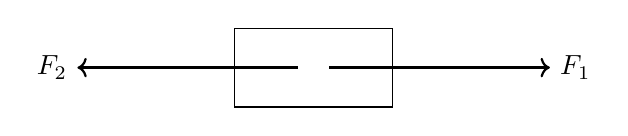
\begin{tikzpicture}

    % Box
    \node[box] (B) at (0,0) {};

    % Forces
    \draw[force] ($(B.center)+(0.2,0)$) -- (3,0) node[right] {$F_1$};
    \draw[force] ($(B.center)+(-0.2,0)$) -- (-3,0) node[left] {$F_2$};

\end{tikzpicture}

\begin{tikzpicture}

    % Box
    \node[box] (B) at (0,0) {};

    % Forces
    \draw[force] ($(B.center)+(0,0.2)$) -- (0,3) node[above] {$F_\text{up}$};
    \draw[force] ($(B.center)+(0,-0.2)$) -- (0,-3) node[below] {$F_\text{down}$};

\end{tikzpicture}


\end{center}
\end{document}